\section{Meetings and Proceedings}
In this section, we detail exactly what happened at select meetings, whose events bear particular significance over the development of our robot.

\subsection{Preseason Overview -- Meeting 1: 2013-08-31}
We held a preseason meeting in order to go over scheduling, recruitment of new members, and hold a quick review of what we learned from our last season. One of the main items we discussed was our scheduling, and as a team we decided to take an aggressive approach towards our first couple of regional competitions in order to secure a place in St. Louis. Because of this, we may need to cut back on scoring the maximum number of points and instead focus on scoring a high, yet consistent number of points. We found out that we need to secure our electronics and work with the field control issues that we were issues. We also plan on placing a much larger emphasis on the CAD design of our robot than we have in our two previous years as it is an efficient way to quickly discover and troubleshoot problems prior to building the system. 

Our final goal is to have two weeks of drive practice before our first regional on December 14th, important for both driver and coaches, to figure out the timing of the game, as well as things that we can or cannot do in game. Organization of the team this year will be facilitated through the use of Google Groups, which will allow all the team members and their parents to be easily contacted for meetings, and will hopefully foster some discussion over build design or game strategy. 

We also decided to meet a few hours after the game was released next week so team members could think about strategies ahead of time and add to the strategy discussion of our first meeting of the season. The meeting was fairly short, but got the team in the right mindset for the upcoming season, and got everyone excited for the  new season!

\newpage \subsection{Initial Design -- Meeting 2: 2013-09-07}
The team decided last week to meet a few hours after the game video and rules were released, so by the time our meeting started, everyone had an idea of how they thought the robot should work, and be built. Fortunately, most team members were on the same page and wanted to focus on scoring as many blocks into the baskets as possible, in a manner that would allow for a integration in the lifting and scoring mechanism. We decided to focus on every aspect of the game for our qualifiers, since it seems like we could consolidate all of the mechanisms into very few.

After a fairly long strategy discussion, some ideas were thrown around as to how to pick up and score the blocks, since we always have a difficult time getting our game pieces, and a rough idea of a mechanism was developed that would use a roller system and a block hopper that would pick up and score the blocks. There is still significant discussion considering the way we will go about constructing a lifting mechanism, with different arguments for and against a rotating arm and a more standard but perhaps less efficient forklift, similar to ``Ring It Up!''. Some of our team members have some experience with constructing forklifts from prior FTC seasons, so we have some idea of what kind of issues we might come across with that kind of design. One thing we discussed was making sure we construct and purchase our materials with a little more regard for quality than we have in previous years, but we wanted to focus on simplicity this season as it worked out very well for us three years ago, and the ideas we are thinking of currently all seem to fit this idea.

Members of the team have assumed different jobs to complete before the next meeting, such as researching lifting mechanisms, getting a BOM for the field and purchasing the materials, and researching the specifications of an IR beacon and sensor, since the team also decided that scoring the block during autonomous is absolutely imperative to the outcome of this game. It is essentially free points that even a defensive robot cannot stop. As of right now we are choosing to focus the endgame period, since lifting and raising the flag are relatively simple tasks. 

We are considering purchasing the AndyMark field, as it would provide us a standardized field and a better replication of the interaction of the robot with the field during competition. 

\newpage \subsection{General Design -- Meeting 3: 2013-09-14}
Today was our second main meeting; we discussed several different raising mechanisms, since we as a team have decided that it was the most important system of our robot.

Our main idea for lifting is an arm that is centered around the top corner. We are designing it to be just long enough to allow us to climb the bar as well as to clear the front block scooper. As for the material, we were looking at Delrin, and wood for our prototype. Delrin has incredible tensile strength. If a material is homogeneous then the tensile and flexural strengths are identical. However, most materials have defects in them which act to concentrate the stresses locally, which in turn cause a localized weakness. We have determined that the flexural strength is greater in the Delrin over the wood as follows. We first see that method for calculating flexural strength is: \[\sigma = \frac{3FL}{2bd^2}\] and we are looking to see which sheet can take in the maximum force, $F$. It directly follows that as we increase $b$, the width measured in in, and $d$, the  thickness measured in in, the sheet can withstand a greater force. Elementary analysis allows us to see that the Delrin is superior than the wood. This will assure us that if our wood prototype works, so should our final design. It will also be able to withstand in competition. 

For the flag spinner, we discussed using some external pins or some type of rubber-esque substance to push against the edge and raise it up. We believe that a rubber-esque material will work. We plan on using 3 NXT motors to provide enough torque and speed to raise the flag. Our goal is to raise the flag in under 5 seconds. 

We also spent a lot of time discussing the importance of autonomous and the structure of our code. We are looking at dynamic autonomous programs that are able to dodge other robots if need be. We are looking forward to prototyping within the next several weeks. Our meetings have mainly comprised of theorizing about code and 3D modeling our robot. We are sharing with the younger students much of the knowledge we have learned over the years as well. 

\newpage \subsection{Initial Field Build -- Meeting 4: 2013-09-21}
Today we began building the field, discussed the lifting, got mail, worked on autonomous theory, cut PVC with safety glasses, and had some fun moving our very mobile robot for a while.  In the mail we received one half of the blocks necessary for the field.
For building we:
\begin{enumerate}
\item Painted the wood
\item Cut all the pvc pipes for the flag spinner
\item Wore safety glasses
\item Cleaned up a lot of pvc dust
\item Screwed temporary screws to the flanges onto the wood
\end{enumerate}

Flag Spinner:
\begin{itemize}
\item Involves NXT motors
\item Gearing 6:1
\item Rubber-esque material did not work out
\item Using extruding pins
\end{itemize}

\newpage \subsection{First Prototype -- Meeting 5: 2013-09-28}
Today was a day for laying out drawings, finalizing designs, and testing some of the flag spinner prototypes. 

We started the day with the usual bit of socialization, before returning to work. The primary topic of discussion is the acquisition mechanism for the blocks. It has been speculated up until this point that we are going to be using a roller, and it looks like those plans may come to fruition. 
We received several items today, including some Tetrix motors, as well as M3 screws and the other half of the blocks.

A to-scale side view drawing shows that the arm we want to design and guiding channels will take up about 7 inches on either side, leaving 8 inches in the middle to mount the block grabbing mechanism on. This fits within our expectations.

It is worth noting that the since we are designing the robot out of raw materials we are using metric, as opposed to the imperial u-channels, so there is some difficulty in lining up the holes if we plan to use any Tetrix. This is a prototype however, and the arm we plan to design for the final design would be out of delrin, and can be designed to fit our needs. The prototype wooden arm also has potential tolerance issues. There is about a 1 block tolerance on the size of the spinning blocks. Stability is key. 

We constructed our first prototype, we assembled the outside arms from plywood. From left to right, there are two arm chasis pieces, the arm pieces and then two arm chasis pieces. The frame design is an A-frame and it works pretty well.

\begin{center}
\begin{figure}[H]
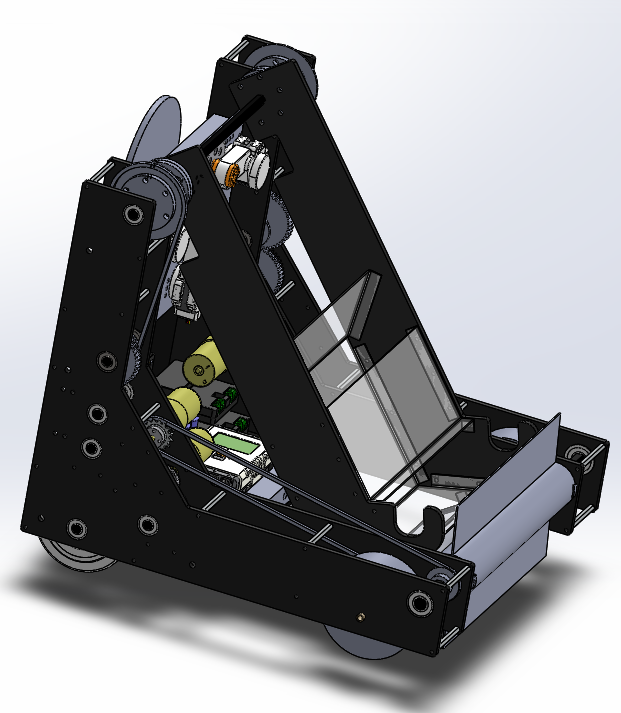
\includegraphics[scale=0.5]{images/RobotV1.png}
\caption{This is the first revision of our Solidworks. We can see the block acquistion device that is essentially a roller that will inhale blocks into our robot}
\end{figure}
\end{center}

Force is not an issue, and remains at a 16:1 ratio with torque gained. It is important to note that the force DOES double when an additional layer is added, however, with the 16:1 ratio between the movement of the bars, the speed with which the bars are raised ALSO doubles. This means that, though the force doubles, the speed at which the arm go up is also doubled. That implies that any torque issue created by adding another layer to the mechanism can be resolved by multiplying the gear ratio of the chain motor by two. The same vertical speed will be achieved.
The prototype is very functional. We connected it to the (makeshift) motor, and ran it. The mechanism lifted very well. The following problems were noted:
\begin{itemize}
\item Block pickup does not work
\item Lifting does not lock after power is lost
\item The wooden shaft collars strip
\item It does not move fast enough
\item It makes the robot very back heavy
\end{itemize}

Possible solutions to these problems (in order) are:
\begin{itemize}
\item Switch from the roller
\item Jam the gears
\item Change the wood to metal
\item Add steel to the front
\end{itemize}

Despite these issues, the lifting mechanism works well, and glides smoothly as long as they aren't stripped. Granted it is currently in prototype form, the final version (which will be produced much more carefully), should be very effective.

We are currently looking into redesigning the block pickup mechanism as it does not seem to be effective. We plan on lowering teh roller to the ground and seeing what happens. 

Currently, our projected maximum height is 32”, just over what we need to hang on the bar.

\newpage \subsection{Flag Spinner Initial Test -- Meeting 6: 2013-10-6}
Today’s meeting was short - it was only two hours. We had a couple ideas we wanted to test, and the tests were successful. We verified our idea would work, and redrew the pictures from two days ago.

The idea we were testing today was whether or not we could raise the flag by using a rubber-like substance to mesh within it and spin. We soon saw that the NXT motors were not as powerful as we would like and the force that the rubber plate was inducing was off center. This makes it unfeasible to use. 

\begin{figure}[H]
\begin{center}
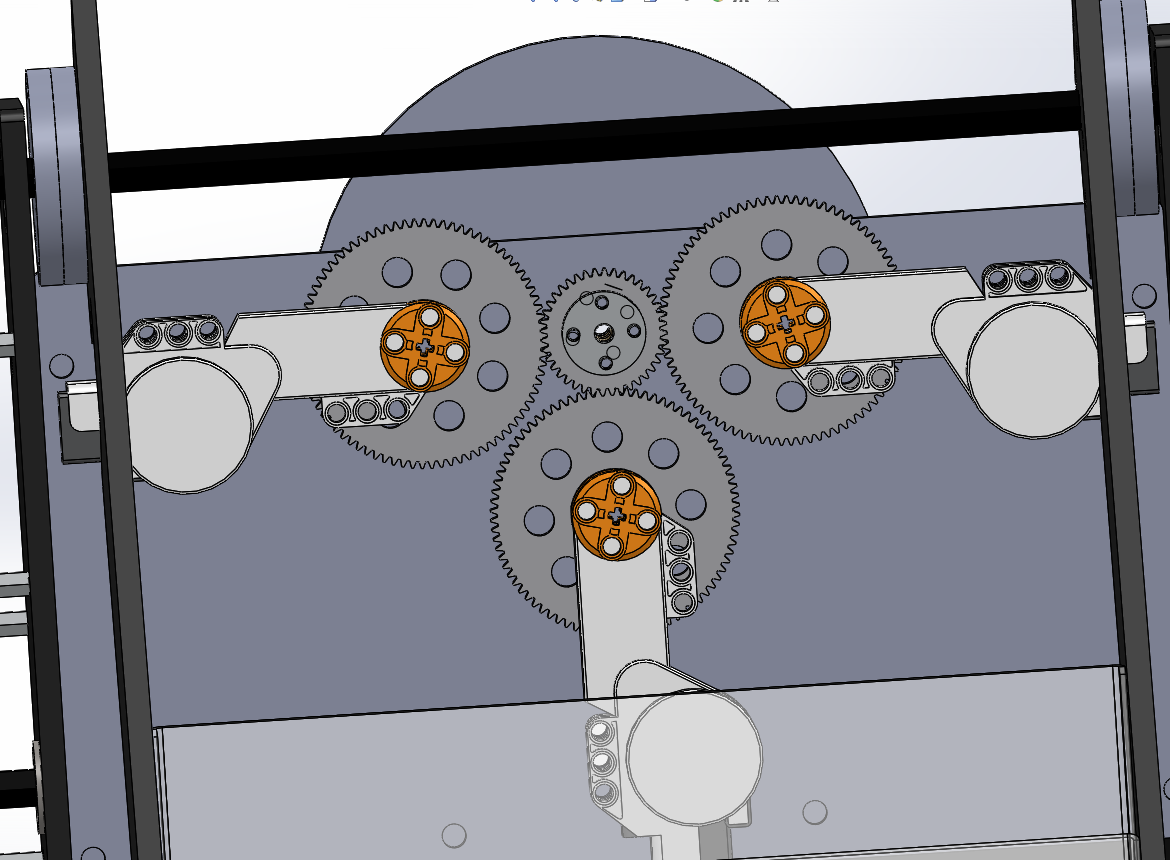
\includegraphics[scale=0.25]{images/FlagSpinnerV1.png}
\end{center}
\end{figure}


We plan on switching to the seemingly common extruded pins design. We plan on having two pins attached off center that are $180^\circ$ apart. We also plan on switching to a Tetrix motor with a $6:1$ gearing ratio. With this ratio, we will be able to raise the flag, theoretically, in under 10 seconds. 

However, this method adds an extra $1.5''$ to our length. As we must stay within the $18''$ length constraint, we may have to shorten our roller (block pickup mechanism). This may become problematic, but as far as we can see we should be able to work around it. 

For the pins, we had two ideas: the first is to use cut Tetrix axles. The second is to use longer Tetrix screws. We plan on using the Tetrix screws first to test and we may end up keeping them on afterwards. 

We also did some more testing with the roller. We experimented with lowering it and shrinking the radius of the aluminum tube. We chose a smaller inner radius due to the fact that it would weigh less and it would be easier to place near the ground. We are still running into issues of picking up much more than 4 blocks at a time. 

We decided on mounting it 1.5'' above the ground because this is just enough to let the blocks slide under as we roll. 

It is the popular idea that we want to completely redesign the block grabbing mechanism due to its inability to give us the accuracy and visibility that we want. Visibility is an issue when we go to the opposite side of the field. 

\newpage \subsection{Block Aquisition Redesign -- Meeting 7: 2013-10-11}
We have spent a lot of time working on scoring blocks, but we overlooked the difficulty of acquiring them. We decided to spend the day looking over our acquisition device as we found it was not very effective. We are looking into changing the roller into a much lower roller made of rubber. We are also looking into changing the entire design altogether. The main ideas consist of driving into blocks and then flipping them into our arm. However, many members of the team do not like the idea of multiple moving parts. 

We decided to extend the final aspect of the roller and found that it was completely ineffective. There is currently no member that continuously supports this idea. 

Today, Garrison proposed that we use a bulldozer like system. A flat plate that we would use to ram into the blocks. Essentially extending our arm to be outside of the frame. We built a first prototype with this and it seems to show some promise. We are still unsure of the implications that this has for the a final working idea. 

Another issue we see with this mechanism is that it is very easy for blocks to slip outside of our robot. 

We currently plan to go home and think about better ideas. We will probably have an in-depth Skype conversation over this idea. We look forward to improving this design as it needs a lot of work. 

The flag spinner was also entirely redesigned as follows:

\begin{figure}[H]
\begin{center}
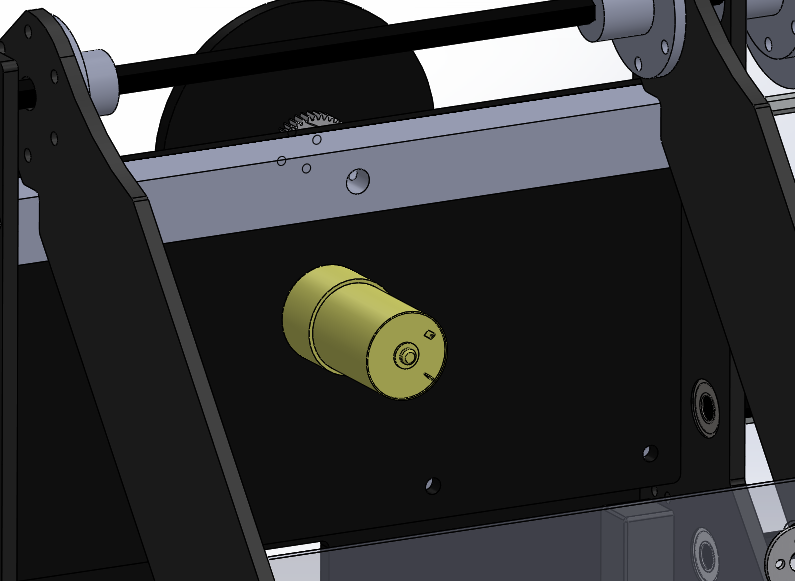
\includegraphics[scale=0.4]{images/FlagSpinnerV2Back.png}
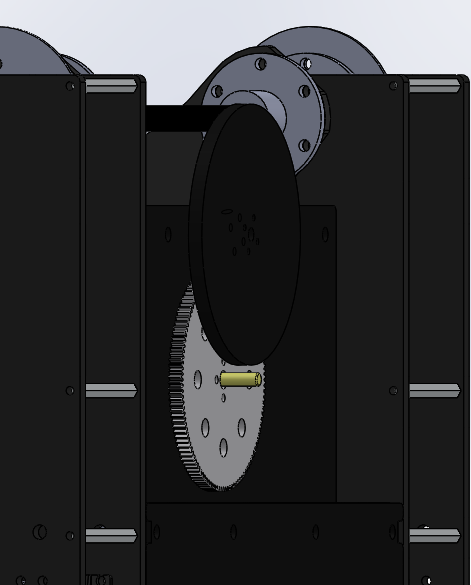
\includegraphics[scale=0.5]{images/FlagSpinnerV2Front.png}
\end{center}
\caption{Here we can see both sides of the new, redesigned, flag spinner. The notable changes include the switch to the Tetrix motor and the removal of the rubber backing in turn for extruding pins (not shown above).}
\end{figure}

\newpage \subsection{Solidworks Redesign -- Meeting 8: 2013-10-18}

After coming back with new ideas, we spent the first hour of our meeting discussing the pros and cons of our new block acquisition mechanism. We all feel that a flat sheet on the ground that we can use to run into the blocks as a bulldozer is the optimal solution. 

We are designing it to be fully flush with the ground. We look forward to testing this out. In solidworks we are redesigning the base of the robot to be shorter to allow the bulldozer system to lie in front. 

\begin{center}
\begin{figure}[h]
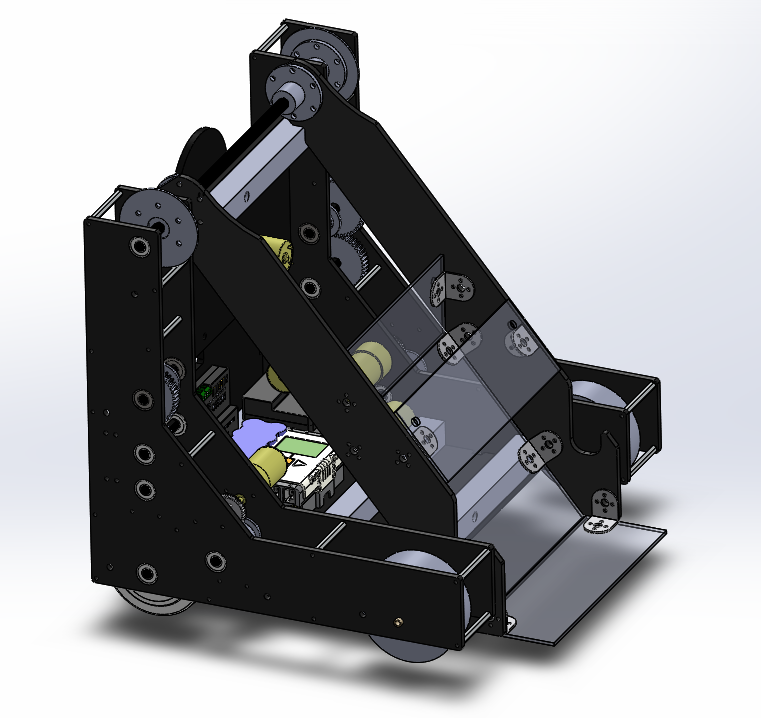
\includegraphics[scale=0.75]{images/RobotV2.png}
\caption{This is the second revision of our Solidworks which includes the redesigned block acquisition device.}
\end{figure}
\end{center}

\newpage \subsection{First Full Test and Match -- Meeting 9: 2013-10-25}

Today was our first day having a fully complete robot. Although we had done several tests of our prototype before, this was the first day we had everything working together. The excitement within our team was immense. We tested our drive train with the added weight of the arm on the motor. We tied the flag mechanism with nylon as our kevlar rope has not yet been received. The kevlar provides less friction and is more like the competition.

Near the bottom, we have a lot of empty space to place the electronics. We hope to use the HiTechnic SuperPro this year to do much more sensor fusion. We want to add an Arduino or Atmel processor (ATUC3b0128) to do much more powerful computation without having to deal with the timing issues that are imposed by using the task system in RobotC and the slow clock of the NXT. We have plans to include gyroscopes, accelerometers and ultrasonic sensors. We are also looking into developing our own infrared seeker, although we are still uncertain about the feasibility of that task. 

With the A-frame design that we have we are able to distribute all of our weight to the back of the robot. This makes it very stable and very difficult to push us. 

When we scored our first block, the entire team was ecstatic. We all felt relief that we were able to lift something and score our blocks. We were somewhat surprised as to how simple it was for us to score a block. It went on just by driving backwards and raising the arm.

The arm went up very smoothly and we had no issues scoring on any of the blocks. We decided to play our first match to see how many points we were able to score.

We gave Tristan the controller and on our first run we were able to score about 200 points. We scored only on the outside baskets. This added up to the balanced bonus bonuses. Overall, we are very happy with the current design of the robot. Although, we do feel that a lot of driver practice is needed, along with an improved block aquisition device. 

Once we had the entire robot built we started testing the arm mechanism and it's ability to remove and score blocks. We found that although it is just in and out straight, moving linearly. We also found that it requires almost no effort to manipulate.

Tristan, our driver, says that with the new Fishtail drive train that we incorporated along with the ease of use of scoring rings and removing them from the ground. We are still unable to consistently pickup 4 blocks. 

There is an air of reminiscence from our first year of FTC. We feel that our strategy and simplicity of our mechanism is very similar. This brings back memories to the members who were on the team from the conception of the team. This also brings an air of confidence among the members about the ability of our robot.

Now there is a lot of talk among the team members about autonomous and strategies for approaching it. We have the ability to determine which column the Infrared beacon is one within one second of our robot starting up.

After we scored our first block and played our first game we decided that we had accomplished a decent amount for this extra Sunday meeting and decided to call it a day. We have high hopes for the competition and expect to place well at our first qualifier. 